\section{Introducción}
\label{introduccion}

Un m\'aser es un \textbf{dispositivo que produce ondas electromagn\'eticas coherentes} mediante la amplificaci\'on por la emisi\'on estimulada de radiaci\'on \cite{maserDefinition}. El t\'ermino se defini\'o como acr\'onimo de \textit{Microwave Amplification by Stimulated Emission of Radiation}.

Como su nombre indica, su funcionamiento está basado en el fenómeno de emisión estimulada de radiación, enunciado por Albert Einstein en 1916.

Una de las principales aplicaciones de los m\'aseres es como relojes at\'omicos de gran precisi\'on, pero tambi\'en se usan como amplificadores, principalmente en radiotelescopios. En secciones posteriores de este documento profundizaremos en las aplicaciones de este tipo de dispositivos.

\subsection{Historia}

El funcionamiento del m\'aser est\'a basado en el fen\'omeno de emisi\'on estimulada de radiaci\'on enunciado por Albert Einstein en 1916. 

En mayo de 1952 Nikolay Basov y Alexander Prokhrov del Instituto de F\'isica de Lebedev describieron el principio del m\'aser en la Academia de Ciencias de la URSS. M\'as tarde, en octubre de 1954  publicaron los resultados de su investigaci\'on.

De forma independiente Charles H. Townes, J. P. Gordon y H. J. Zeiger fabricaron en 1953 en la Universidad de Columbia el primer m\'aser. Este dispositivo utilizaba un haz de mol\'eculas de amon\'iaco para producir la amplificaci\'on de microondas a la frecuencia de 24 GigaHerzios.

M\'as tarde Townes trabaj\'o con Arthur L. Schawlow para describir el principio del m\'aser \'optico o l\'aser, y en 1958 hicieron varias publicaciones sobre este tema, aunque por aqu\'el entonces no siguieron con las investigaciones en ese campo.

En 1959 Townes y Schawlow obtuvieron una patente del m\'aser. Este dispositivo se usaba para amplificar se\~nales de radio y como detector ultrasensible para investigaci\'on espacial.

En 1964 Townes, Basov y Prokhorov recibieron el premio Nobel de F\'isica por su trabajo en este campo. A Townes se le adjudic\'o la mitad del premio y la otra mitad se reparti\'o entre Basov y Prokhorov.

\begin{figure}[h]
\begin{center}$
\begin{array}{ccc}
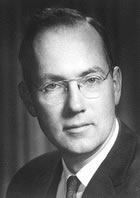
\includegraphics[width=0.25\textwidth]{./Utils/townes.jpg} &
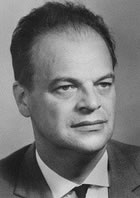
\includegraphics[width=0.25\textwidth]{./Utils/basov.jpg} &
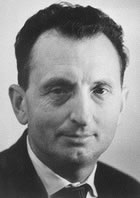
\includegraphics[width=0.25\textwidth]{./Utils/prokhorov.jpg}
\end{array}$
\end{center}
\caption{Townes, Basov y Prokhorov, de izquierda a derecha}
\end{figure}

En 1965 se descrubri\'o el primer m\'aser astron\'omico en la nebulosa de Ori\'on. Era un m\'aser de hidroxilo, que emite radiaci\'on en varias longitudes de onda, aunque las m\'as utilizadas son las de 18cm (1,7GHz de frecuencia).
\subsection{Terminolog\'ia}

Aunque el t\'ermino \textit{MASER} se difini\'o como acr\'onimo de \textbf{Microwave Amplification by Stimulated Emission of Radiation}, con el tiempo y el avance de la tecnolog\'ia este t\'ermino se ha ido quedando obsoleto, y se ha empezado a llamar al dispositivo \textit{m\'aser} en min\'usculas, y ya no en forma de acr\'onimo. 

El motivo por el que la definici\'on ya no es precisa es debido a que el rango de frecuencias de funcionamiento de los m\'aseres actuales no est\'a limitado al de microondas, sino que se extiende en el espectro. Por este motivo el f\'isico Charles H. Townes, quien le hab\'ia dado el nombre original junto con sus colaboradores, sugiri\'o sustituir la palabra ``microondas'' por ``molecular'' en la definici\'on. Otros cient\'ificos, sin embargo, alegaron que con este intento de extender el acr\'onimo Charles H. Townes estaba intentando darle m\'as importancia a su descubrimiento y aumentar su reputaci\'on en el mundo cient\'ifico.

Cuando se desarroll\'o el l\'aser en 1957, Townes, Schawlow y sus colegas de Bell Labs impulsaron la adopci\'on del t\'ermino \textit{m\'aser \'optico}, pero \'este fue sustituido por \textit{l\'aser} (Light Amplification by Stimulated Emission of Radiation), nombre defendido por Gordon Gould. De hecho Gould propuso un nombre diferente para los dispositivos que emit\'ian en cada regi\'on del espectro. As\'i, habr\'ia \textit{grasers} (``gamma ray lasers''), \textit{xasers} (``x-ray lasers''), \textit{uvasers} (``ultraviolet lasers''), \textit{lasers} (``visible lasers''), \textit{iraser} (``infrared lasers''), \textit{masers} (``microwave masers'') y \textit{rasers} (``RF masers''). La mayor parte de estos nombres, sin embargo, nunca llegaron a adoptarse, y todos se han quedado obsoletos excepto \textit{\textbf{m\'aser}} y \textit{\textbf{l\'aser}}.

Actuamente se denomina \textit{l\'aser} al dispositivo que emite en la regi\'on del espectro delimitada por los rayos-X y los infrarrojos, y \textit{\textbf{m\'aser}} al que \textbf{emite en la regi\'on de microondas e inferiores}. 
